\documentclass{beamer}
\setbeamertemplate{footline}[page number]
\date{}
\author{}
\institute{}

%%%%%%% Put these names back in the final version 
%\\Aswathy Rajendra Kurup\\Meenu Ajith}
%\institute{Department of Electrical and Computer Engineering\\The University of New Mexico}
\setbeamercovered{transparent}
\usepackage{setspace}
\usepackage{array}
\usepackage[T1]{fontenc}
\usepackage{graphicx}
\usepackage{amsmath}
\usepackage{amsfonts}
\usepackage{amssymb}
\usepackage{makeidx}
\usefonttheme{serif}
\usepackage{multirow}
\usepackage{booktabs} 
\usepackage{rotating}
\usepackage{color}
\usepackage{float}
\usepackage[latin1]{inputenc}
\usepackage[english]{babel}
\usepackage{amsmath}
\usepackage{amsfonts}
\usepackage{eurosym}
\usepackage{rotating}
\usepackage{multicol}
\usepackage{pythonhighlight}
\usepackage[normalem]{ulem}
\newcommand{\ba}{{\bf a}}
\newcommand{\bb}{{\bf b}}
\newcommand{\bc}{{\bf c}}
\newcommand{\bd}{{\bf d}}
\newcommand{\be}{{\bf e}}
\newcommand{\bbf}{{\bf f}}
\newcommand{\bg}{{\bf g}}
\newcommand{\bh}{{\bf h}}
\newcommand{\bi}{{\bf i}}
\newcommand{\bk}{{\bf k}}
\newcommand{\bl}{{\bf l}}
\newcommand{\bm}{{\bf m}}
\newcommand{\bn}{{\bf n}}
\newcommand{\bo}{{\bf o}}
\newcommand{\bp}{{\bf p}}
\newcommand{\bq}{{\bf q}}
\newcommand{\br}{{\bf r}}
\newcommand{\bs}{{\bf s}}
\newcommand{\bt}{{\bf t}}
\newcommand{\bu}{{\bf u}}
\newcommand{\bv}{{\bf v}}
\newcommand{\bw}{{\bf w}}
\newcommand{\bx}{{\bf x}}
\newcommand{\by}{{\bf y}}
\newcommand{\bz}{{\bf z}}

\newcommand{\bA}{{\bf A}}
\newcommand{\bB}{{\bf B}}
\newcommand{\bC}{{\bf C}}
\newcommand{\bE}{{\bf E}}
\newcommand{\bG}{{\bf G}}
\newcommand{\bH}{{\bf H}}
\newcommand{\bI}{{\bf I}}
\newcommand{\bK}{{\bf K}}
\newcommand{\bL}{{\bf L}}
\newcommand{\bM}{{\bf M}}
\newcommand{\bO}{{\bf O}}
\newcommand{\bQ}{{\bf Q}}
\newcommand{\bR}{{\bf R}}
\newcommand{\bS}{{\bf S}}
\newcommand{\bT}{{\bf T}}
\newcommand{\bV}{{\bf V}}
\newcommand{\bW}{{\bf W}}
\newcommand{\bX}{{\bf X}}
\newcommand{\bY}{{\bf Y}}
\newcommand{\bZ}{{\bf Z}}
\newcommand\uptocnt{\stackrel{\mathclap{\normalfont\mbox{c}}}{\propto}}
\newcommand{\bpt}{{\bf pt}}
\newcommand{\bpl}{{\bf pl}}
\newcommand{\bdp}{{\bf dp}}
\newcommand{\btemp}{{\bf temp}}

\newcommand{\bmu}{{\boldsymbol \mu}}
\newcommand{\bSigma}{{\boldsymbol \Sigma}}
\newcommand{\bsigma}{{\boldsymbol \sigma}}
\newcommand{\bvarPhi}{{\boldsymbol \varPhi}}
\newcommand{\bvarphi}{{\boldsymbol \varphi}}
\newcommand{\bPhi}{{\boldsymbol \Phi}}
\newcommand{\bdelta}{{\boldsymbol \delta}}
\newcommand{\bZero}{{\bf 0}}
\newcommand{\bOne}{{\bf 1}}
\newcommand{\balpha}{{\boldsymbol \alpha}}
\newcommand{\bAlpha}{{\boldsymbol A}}
\newcommand{\btheta}{{\boldsymbol \theta}}

\newcommand{\softmax}{\text{softmax}}
\newcommand{\diag}{\text{diag}}
\newcommand{\sinc}{\mathrm{sinc}}
\newcommand{\argmin}{\mathop{\mathrm{argmin}}}
\newcommand{\infl}{\eta}
\newcommand{\Ind}{\mathrm{I}}
\newcommand{\Real}{\mathbb R}
\newcommand{\Intg}{\mathbb Z}
\newcommand{\Complex}{\mathbb C}
\newcommand{\Natural}{\mathbb N}
\newcommand{\Fourier}[1]{\mathcal{F} \{#1\}}
%\newcommand{\ii}{\mathbbm{i}}
\newcommand{\bphi}{\boldsymbol{\mathit{\phi}}}

\newcommand{\hs}{\hspace{2pt}}
\newcommand{\sign}{\text{sign}}
\author{Manel Mart\'inez-Ram\'on\\Meenu Ajith\\Aswathy Rajendra Kurup}

\usetheme{Madrid}
\usecolortheme{beaver}
\usepackage{tikz}
\usetikzlibrary{fit,arrows,calc,positioning}
\usepackage{listings}
\usepackage{xcolor}
\usepackage{emerald} 
\usepackage[T1]{fontenc} 
\usepackage{verbatim}
\usepackage{graphicx}
\usepackage{epsfig}
\usepackage{psfrag}
\usepackage[english]{babel}
\usepackage{listings}
\usepackage{courier}
\usepackage{color}
 \usepackage{vwcol} 
 \usepackage[english]{babel} % To obtain English text with the blindtext package
\usepackage{blindtext}
\definecolor{codegreen}{rgb}{0,0.6,0}
\definecolor{codegray}{rgb}{0.5,0.5,0.5}
\definecolor{codepurple}{rgb}{0.58,0,0.82}
\definecolor{backcolour}{rgb}{0.95,0.95,0.92}

\lstdefinestyle{mystyle}{
  backgroundcolor=\color{backcolour},   commentstyle=\color{codegreen},
  keywordstyle=\color{magenta},
  numberstyle=\tiny\color{codegray},
  stringstyle=\color{codepurple},
  basicstyle=\ttfamily\footnotesize,
  breakatwhitespace=false,         
  breaklines=true,                 
  captionpos=b,                    
  keepspaces=true,                 
  numbers=left,                    
  numbersep=5pt,                  
  showspaces=false,                
  showstringspaces=false,
  showtabs=false,                  
  tabsize=2
}
\lstset{style=mystyle}

%% Stuff for movies

% %\newcommand{\bt}{{\bf t}}
% \newcommand{\br}{{\bf r}}
% \newcommand{\bs}{{\bf s}}
% \newcommand{\by}{{\bf y}}
% \newcommand{\bz}{{\bf z}}
% \newcommand{\bx}{{\bf x}}
% \newcommand{\bw}{{\bf w}}
% \newcommand{\be}{{\bf e}}
% \newcommand{\bbf}{{\bf f}}
% \newcommand{\bb}{{\bf b}}
% \newcommand{\bd}{{\bf d}}
% \newcommand{\bA}{{\bf A}}
% \newcommand{\bB}{{\bf B}}
% \newcommand{\bL}{{\bf L}}
% \newcommand{\bM}{{\bf M}}

% \newcommand{\bC}{{\bf C}}
% \newcommand{\bI}{{\bf I}}
% \newcommand{\bK}{{\bf K}}
% \newcommand{\bk}{{\bf k}}
% \newcommand{\bT}{{\bf T}}
% \newcommand{\bV}{{\bf V}}
% \newcommand{\bW}{{\bf W}}
% \newcommand{\bX}{{\bf X}}
% \newcommand{\bY}{{\bf Y}}
% \newcommand{\bZ}{{\bf Z}}
% \newcommand{\bm}{{\bf m}}
% \newcommand{\bpt}{{\bf pt}}
% \newcommand{\bpl}{{\bf pl}}
% \newcommand{\bdp}{{\bf dp}}
% \newcommand{\btemp}{{\bf temp}}
% \newcommand{\bl}{{\bf l}}
% \newcommand{\bu}{{\bf u}}
% \newcommand{\bmu}{{\boldsymbol \mu}}
% \newcommand{\bSigma}{{\boldsymbol \Sigma}}
% \newcommand{\bLambda}{{\boldsymbol \Lambda}}

% \newcommand{\bsigma}{{\boldsymbol \sigma}}
% \newcommand{\bvarphi}{{\boldsymbol \varPhi}}
% \newcommand{\btheta}{{\boldsymbol \theta}}
% \newcommand{\bZero}{{\bf 0}}
% \newcommand{\balpha}{{\boldsymbol \alpha}}
% \newcommand{\bpi}{{\boldsymbol \pi}}
% \newcommand{\bxi}{{\boldsymbol \xi}}
% \newcommand{\bdelta}{{\boldsymbol \delta}}
\lstset{
	language=Python,
	basicstyle=\footnotesize\ttfamily\color{black},
	commentstyle = \footnotesize\ttfamily\color{red},
	keywordstyle=\footnotesize\ttfamily\color{blue},
	stringstyle=\footnotesize\ttfamily\color{black},
%	columns=fixed,
%	numbers=left,    
	numberstyle=\tiny,
	stepnumber=1,
	numbersep=5pt,
	tabsize=1,
	extendedchars=true,
	breaklines=true,            
	frame=b,         
	showspaces=false,
	showtabs=true,
	xleftmargin=6pt,
	framexleftmargin=6pt,
	framexrightmargin=2pt,
	framexbottommargin=4pt,
	showstringspaces=false      
}

\lstloadlanguages{
         Python
}

%\graphicspath{ {./images/} }  % Figures path - used in graphicx

%\selectcolormodel{cmyk}

\mode<presentation>

\newcommand{\dred}{darkred!90!black}
\newcommand{\written}{\ECFJD\textcolor{cyan!50!white}}
\newcommand{\hlight}{\textcolor{\dred}}
\newcommand{\Ex}{\textcolor{\dred}{Ex. }}

% remove navigation symbols in full screen mode
\setbeamertemplate{navigation symbols}{}  
\setbeamertemplate{blocks}[rounded][shadow=false]
\setbeamercolor{note page}{fg=black}

\setbeamercolor{title}{fg=\dred}
\setbeamercolor{frametitle}{fg=white}
\setbeamercolor{frametitle}{bg=\dred}
\setbeamercolor{structure}{fg=black,bg=white}
\setbeamercolor{background canvas}{bg=white,fg=black}
\setbeamercolor{normal text}{fg=black,bg=white}
\setbeamercolor{item}{fg=red!80!black,bg=white!}
\addtobeamertemplate{block begin}{\setbeamercolor{block title}{fg=white,bg=\dred}
\setbeamercolor{block body}{fg=white,bg=gray}}{}


\title{6. Attention-based networks}
\subtitle{6.1. Attention mechanisms}

\addtobeamertemplate{frametitle}{}


\begin{document}
\maketitle


\begin{frame}{Introduction}
\begin{itemize}
\item  Attention is a core human brain functioning mechanism and a complex cognitive function.
\item Attention is the ability to concentrate on information parts and not as a whole. 
\item For example, humans tend to focus on specific parts or aspects of a scene and to identify  similarities with other scenes. 
\item Humans process information by selecting high-value features from  huge information sources with limited resources. 
\item Attention networks are inspired by this behavior.
\item From 2020 or so, the dominant models for all the natural language processing tasks. It is based on a form of attention mechanism.  
\end{itemize}
\end{frame}

\begin{frame}{Attention pooling}
\begin{itemize}
    \item An attention mechanism is a system to access a dataset $\mathcal{D}$ consisting of a set of tuples key-value $\bk_i, \bv_i$ through a query $\bq$. 
    \begin{equation}
        \text{Attention}\left(\bq,\mathbb{D} \right) = \sum_{i=1}^N \alpha\left(\bq,\bk_i\right) \bv_i
    \end{equation}
    where $\alpha\left(\bq,\bk_i\right) \in \mathbb{R}$  are called \emph{attention weights} and they measure the relevance of a key to the query. 
    \item The weights are normalized so they produce a convex combination, i.e,
    \begin{equation}
        \sum_{i=1}^N \alpha\left(\bq,\bk_i\right) = 1
    \end{equation}
\end{itemize}
\end{frame}

\begin{frame}{Attention pooling}
    \begin{itemize}
        \item A particular form of the weights useful in deep learning is
        \begin{equation}
            \alpha\left(\bq,\bk_i\right) = \frac{\exp\left(f\left( \bq, \bk_i \right)\right)}{\sum_{j=1}^N \exp\left(f\left( \bq, \bk_j \right)\right)}
        \end{equation}
where $f(\cdot)$ is any function useful to measure some similarity between the query and the key.  
\item This function is itself a softmax activation and it has properties of probability mass function. 
\end{itemize}
\end{frame}

\begin{frame}{Attention pooling}
\begin{center}
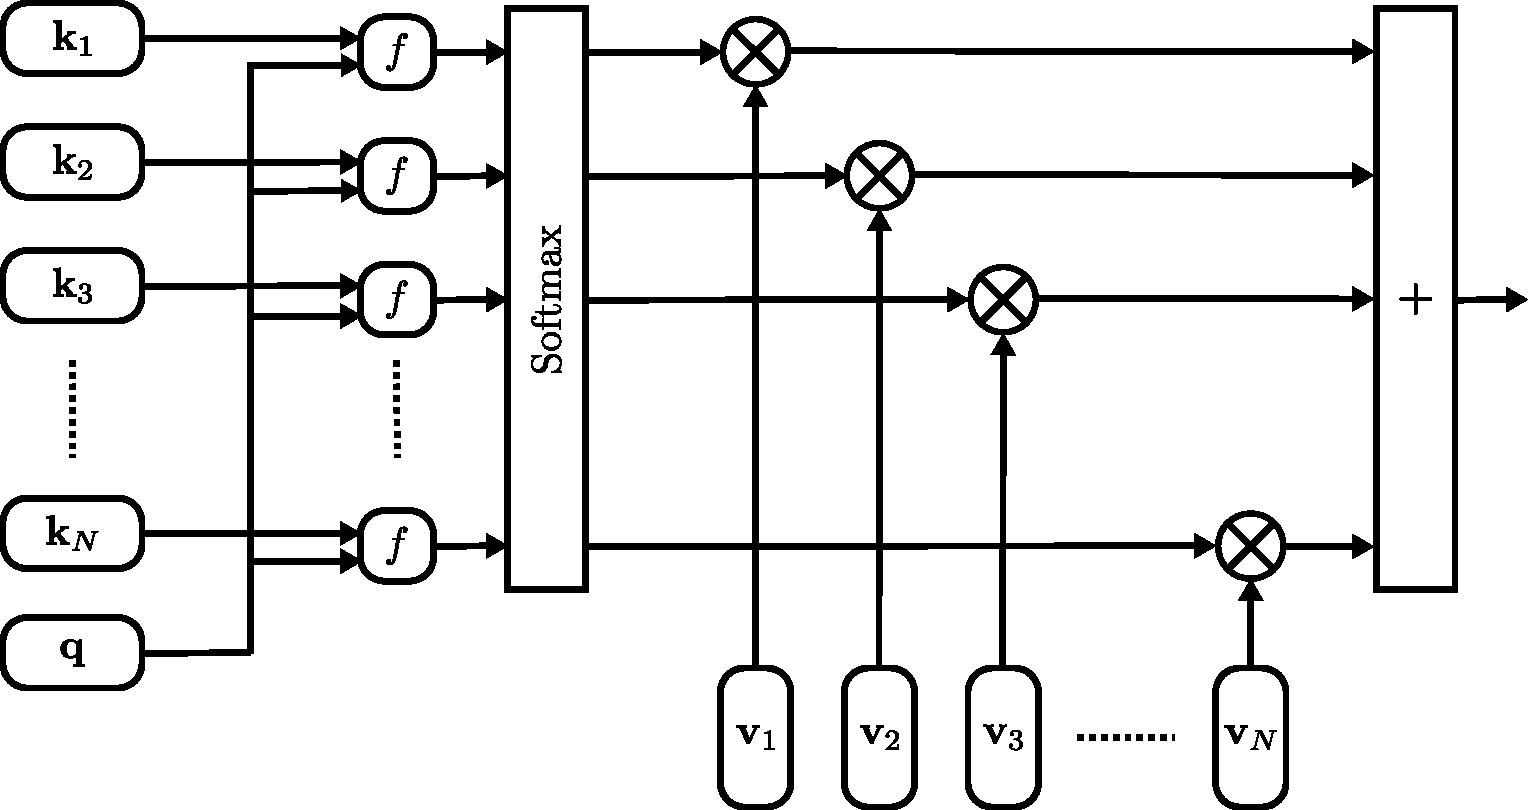
\includegraphics[scale=0.4]{Module 6 (Attention-based networks)/pics/attention.pdf}

Attention pooling as a convex combination of values.
\end{center} 
\end{frame}

\begin{frame}{Attention pooling}{Nadaraya-Watson Regression}
\begin{itemize}
    \item A regression machine can be constructed as an attention-pooling mechanism 
    \begin{equation}
        g(x) = \sum_{i=1}^N y_i \frac{f(x,x_i)}{\sum_{j=1}^N f(x,x_j)} 
    \end{equation}
\item Regression $g(x)$   as $x$ as the query, and the keys are training samples $x_i$. The values are regressors $y_i$. 
\end{itemize}
\end{frame}
\begin{frame}{Attention pooling}{Nadaraya-Watson Regression}
\begin{itemize}
    \item Function $y = 2 sin(x) + x + \varepsilon$ is to be approximated with the N-W regressor, where $\varepsilon_i$ is a Gaussian noise of zero mean and unit variance. 
    \item The training data consists of 100 samples distributed uniformly in the interval $0 \sim 4$.
    \item The performance is compared wrt the following kernels: 
\end{itemize}
\begin{equation}
\begin{split}\begin{aligned}
f(\mathbf{q}, \mathbf{k}) & = \exp\left(-\frac{1}{2} \|\mathbf{q} - \mathbf{k}\|^2 \right) && \mathrm{Gaussian} \\
f(\mathbf{q}, \mathbf{k}) & = 1 \text{ if } \|\mathbf{q} - \mathbf{k}\| \leq 1 && \mathrm{Boxcar} \\
f(\mathbf{q}, \mathbf{k}) & = \mathop{\mathrm{max}}\left(0, 1 - \|\mathbf{q} - \mathbf{k}\|\right) && \mathrm{Epanechikov}
\end{aligned}\end{split}
\end{equation}
   
\end{frame}

\begin{frame}{Attention pooling}{Nadaraya-Watson Regression}
\vspace{-1cm}
 \begin{center}
 Comparisons of different kernels.
        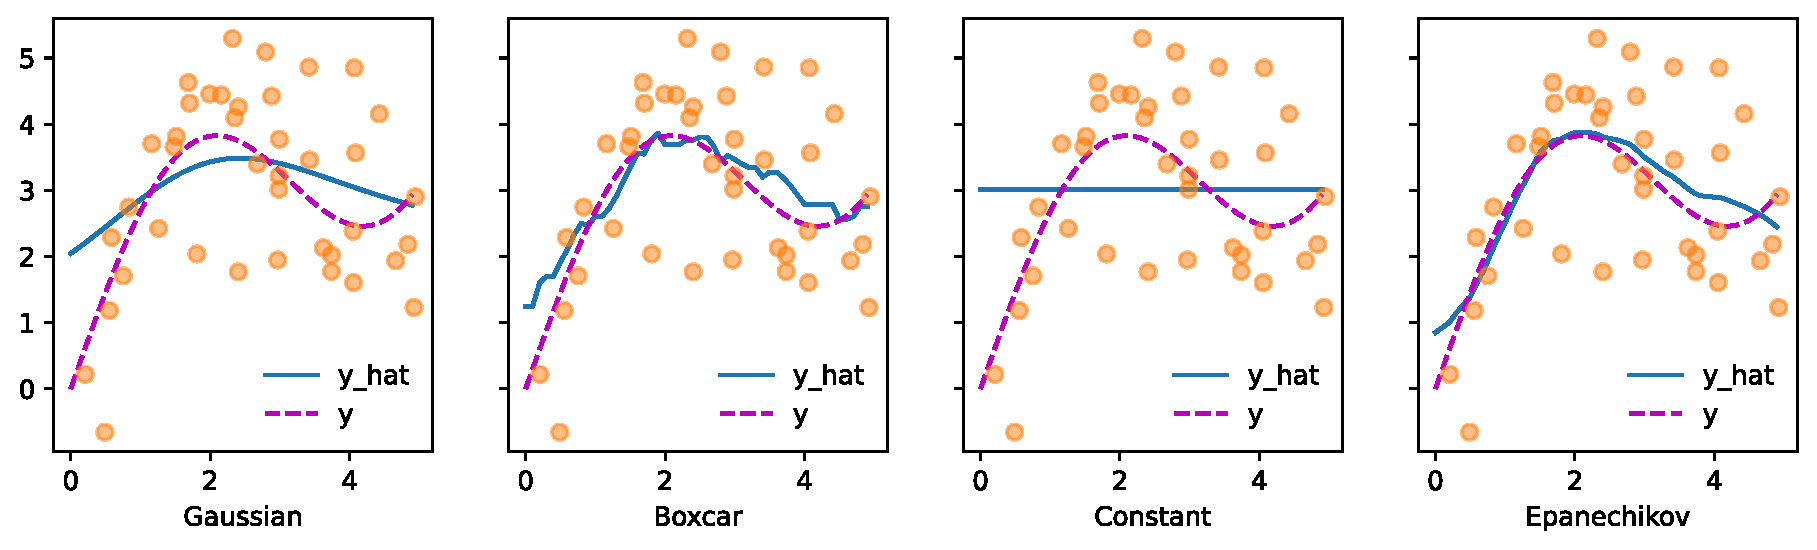
\includegraphics[scale=0.3]{Module 6 (Attention-based networks)/pics/output_attention-pooling_d5e6b2_67_0.pdf}
    \end{center}

    \begin{center}
    Results of the Gaussian kernel with different width parameters. 
        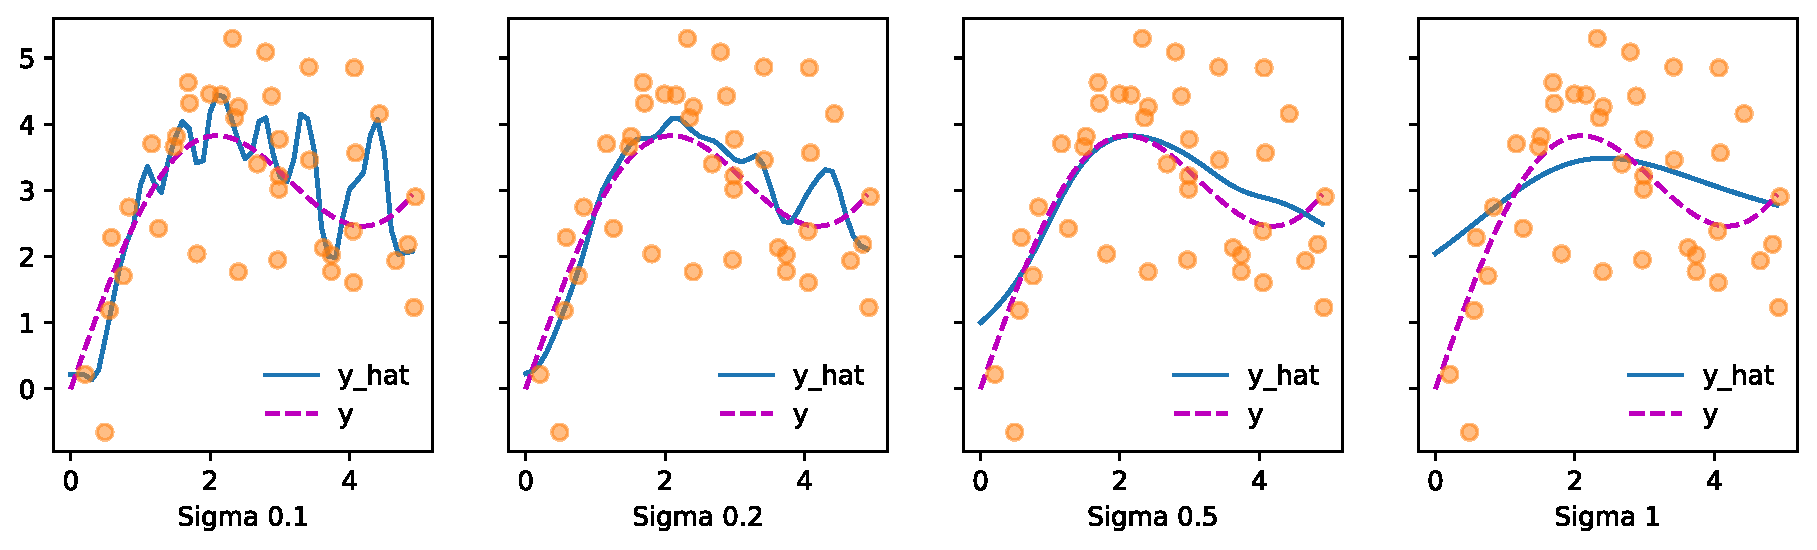
\includegraphics[scale=0.3]{Module 6 (Attention-based networks)/pics/output_attention-pooling_d5e6b2_97_0.pdf}
    \end{center}
\footnotesize{Zhang, Lipton, Li, Smola. 
\href{http://d2l.ai/chapter_attention-mechanisms-and-transformers/attention-pooling.html}{{\color{blue}Dive Into Deep Learning}}, 2023}
\end{frame}



\begin{frame}{Attention functions}
{Dot product}
\begin{itemize}
\item Euclidian distance
\begin{equation}
    f\left(\bq,\bk \right) =-\|\bq-\bk\|^2 = \|\bq\|^2 - \|\bk\| +2\bq^\top \bk
\end{equation}
If we assume that the norm of the keys are approximately constant, and taking into account that $\bq$ is the same for all keys 
\begin{equation}
    f\left(\bq,\bk \right) =2\bq^\top \bk + \text{constant}
\end{equation}
\item We can normalize the dot product with respect to the dimension $D$ of the vectors and apply a softmax:
\begin{equation}
    \alpha\left(\bq, \bk_i \right) = \frac{\exp\left(D^{-\frac{1}{2}}\bq^\top \bk_i\right)}{\sum_{j=1}^N \exp\left(D^{-\frac{1}{2}}\bq^\top \bk_j\right)}
\end{equation}

\end{itemize}
    
\end{frame}
\begin{frame}{Attention functions}{Dot product}
\begin{itemize}
\item The attention mechanism input to the sum block of slide 5 can be written as
\begin{equation}
\bz =\bV^\top \softmax \left( D^{\frac{1}{2}} \bq^\top \bK \right) 
\end{equation}
where $\bK$ contains all the keys and $\bV$ all the values.


\item In practice, the query and the key do not have the same dimension, therefore, transformation matrices are used:

\begin{equation}
    \bz =\bV^\top  \softmax \left( D^{\frac{1}{2}} \bq^\top \bM \bK \right) \in \mathbb{R}^N
\end{equation}
where $\bM \in \mathbb{R}^{D_q \times D_k}$ transforms from the space of queries to the one of keys.
 \end{itemize}   
\end{frame}
\begin{frame}{Attention functions}{Dot product}
\begin{itemize}
    \item If $\bQ$ contains a set of $M$ queries, we can construct a set of responses as
\begin{equation}
    \bZ =\bV^\top  \softmax \left( D^{\frac{1}{2}} \bQ^\top \bM \bK \right) \in \mathbb{R}^{N\times M}
\end{equation}
\item This is necessary for training purposes by using mini batches. 
\end{itemize}
\end{frame}

\begin{frame}{Additive attention}
\begin{itemize}
    \item The additive attention function also assumes that the query and the key have different lengths. The  scoring, in this case, is
    \begin{equation}\label{eq:additive_attention}
         f\left(\bq,\bk \right) = \bw_f \tanh \left( \bW_q^\top \bq + \bW_k^\top \bk\right)
    \end{equation}

 \item Matrices $\bW_q$ and $\bW_k$, and vector $\bw_f$ are trainable parameters. Therefore, this is equivalent to a dense or fully connected network with one hidden layer with tanh activation and one linear scalar output.
 \end{itemize}
\end{frame}

\begin{frame}{Attention mechanisms}{The Badanau Attention Mechanism}
\begin{itemize}
    \item Recall the RNN sequence to sequence machine translation. 
    \begin{center}
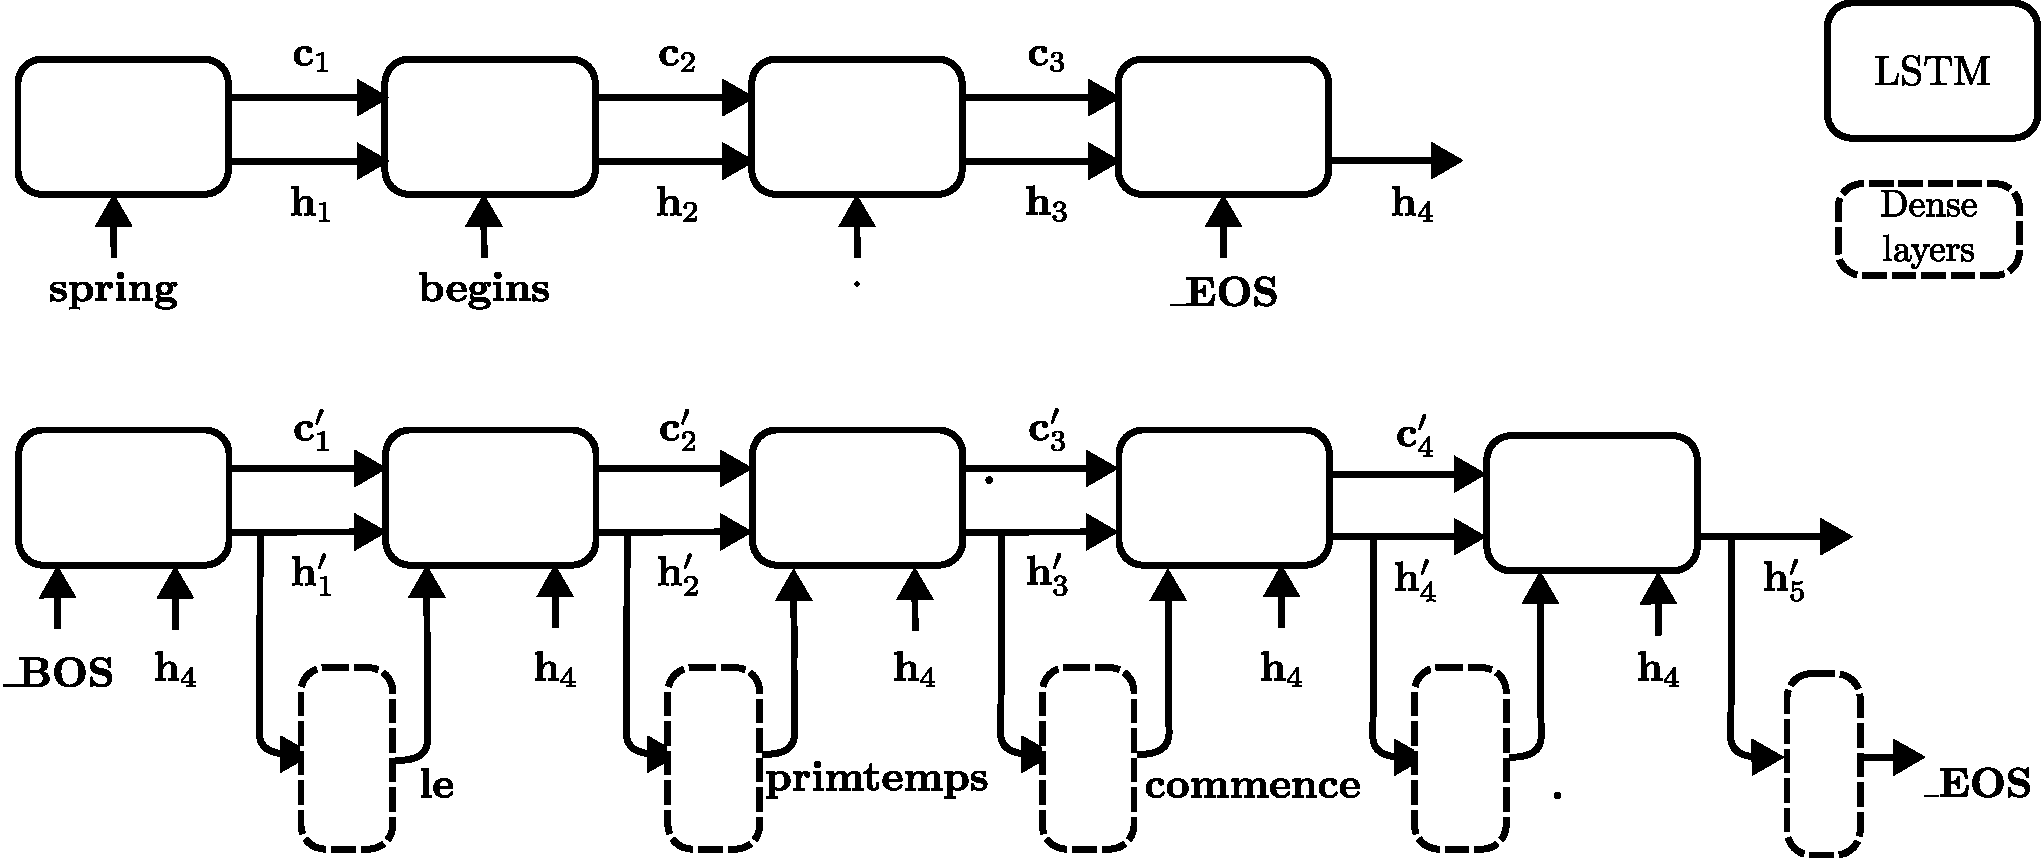
\includegraphics[scale= 0.3]{Module 6 (Attention-based networks)/pics/sequence_translate_RNN_detailed.pdf}
  \end{center}
\end{itemize}
\end{frame}

\begin{frame}{Attention mechanisms}{The Badanau Attention Mechanism}
\begin{multicols}{2}
\begin{center}
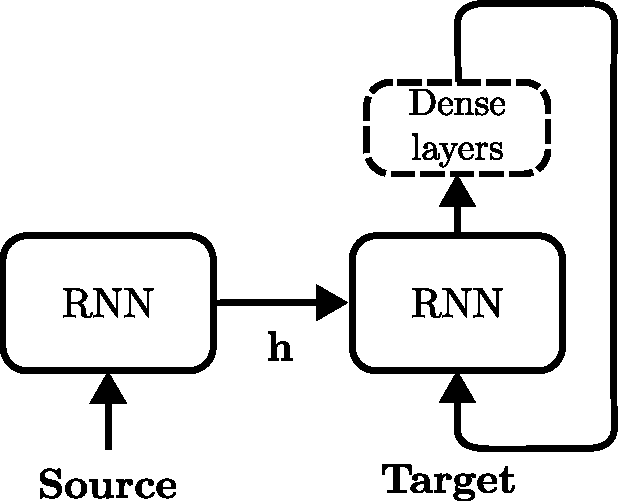
\includegraphics[scale=0.3]{Module 6 (Attention-based networks)/pics/sequence_translate_RNN_compact.pdf}
\end{center}
\columnbreak
\begin{itemize}
\item The main limitation of this method is the length of states $\bh$. There may be not enough space to code long sequences. 
\end{itemize}  

\end{multicols}
\begin{itemize}
    \item This limitation can be overcome with the use of attention mechanisms: when a token is predicted, a model attends only to parts of the input sequence that are relevant to the prediction. 
    \item These parts are then used to modify the state before producing the next prediction.
    \item This gave rise to the idea of transformers. 
\end{itemize}
\end{frame}
\begin{frame}{Attention mechanisms}{The Badanau Attention Mechanism}
\begin{itemize}
    \item The encoder RNN passes states $\bh_t$ to the decoder. The decoder updates its states at every step with an attention pooling.
\end{itemize}
\begin{multicols}{2}
    \begin{center}
        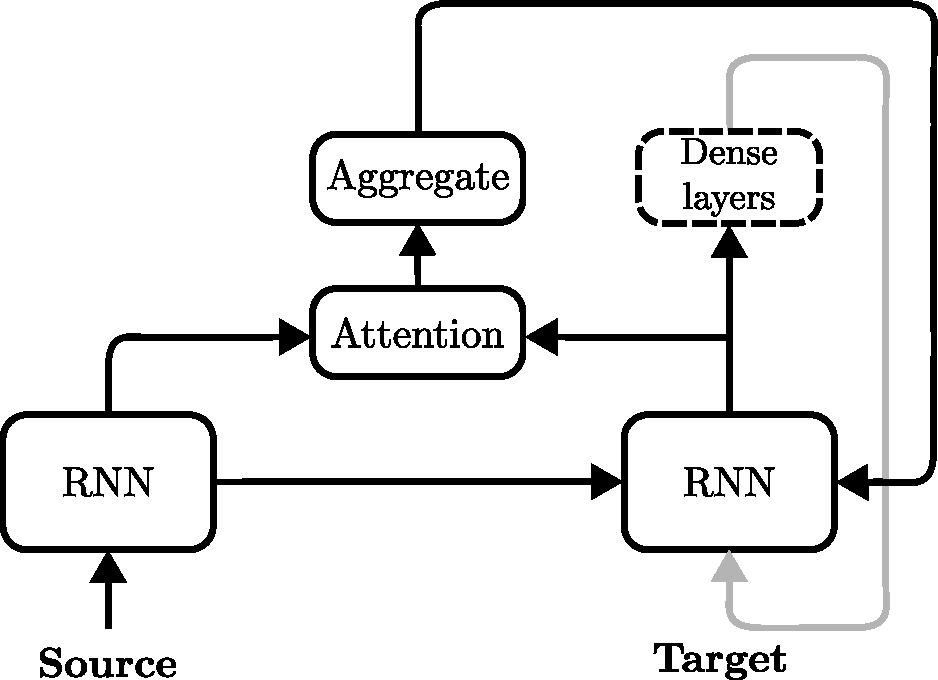
\includegraphics[scale=0.3]{Module 6 (Attention-based networks)/pics/sequence_translate_RNN_Bahdanau_compact.pdf}
    \end{center}
\columnbreak
\begin{itemize}
\item If $\bh'_{t'}$ are the states of the decoder
\end{itemize}
\begin{equation}
    \bc_{t'} = \sum_{t=1}^T \alpha\left(\bh'_{t'-1},\bh_t  \right)\bh_t
\end{equation}
\begin{itemize}
    \item Then, $\bc_t'$ is passed to the dense block to generate the next state $\bh'_{t'}$ and a new token.
\end{itemize}
\end{multicols}
\begin{itemize}
\item The additive attention scoring in Eq. \eqref{eq:additive_attention} is used.
\end{itemize}
\end{frame}

\begin{frame}{Multi head attention}
\begin{itemize}
    \item The multi-head attention combines different behaviors of the same attention mechanism into a feature space.
    \item The responses are linearly combined at the output.
\end{itemize}
\begin{center}
    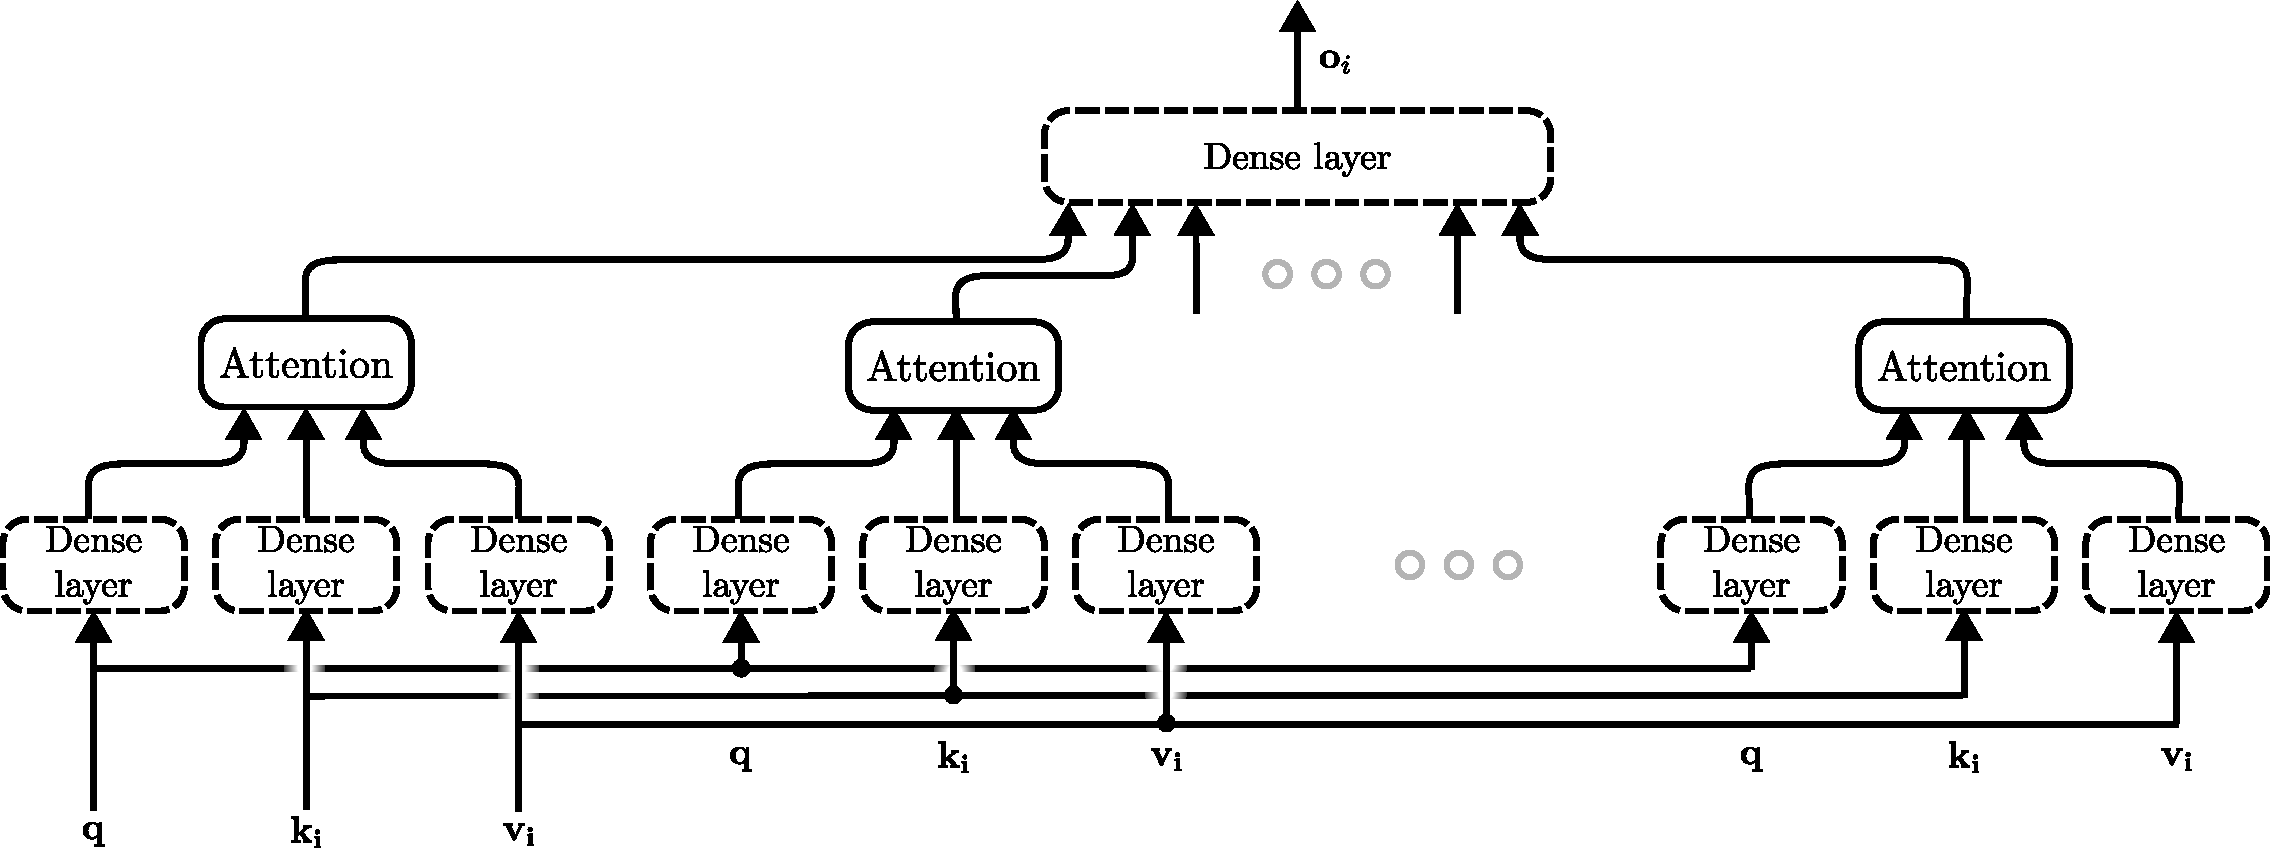
\includegraphics[scale=0.3]{Module 6 (Attention-based networks)/pics/multihead_attention.pdf}
\end{center}
    \begin{equation}
        \bh_{i,j} = f\left({\bW^{(q)}_j}^\top \bq_i,{\bW^{(k)}_j}^\top \bk_i, {\bW^{(v)}_j}^\top \bv_i    \right), ~~~~\bo_i=\sum_j {\bw_j^{(o)}}^\top \bh_{i,j}
    \end{equation}
\end{frame}

\end{document}
